\documentclass[tikz,border=6pt]{standalone}
\usepackage{xcolor}
\begin{document}
% Canonical ch-diagram for 8_1^-1,-1
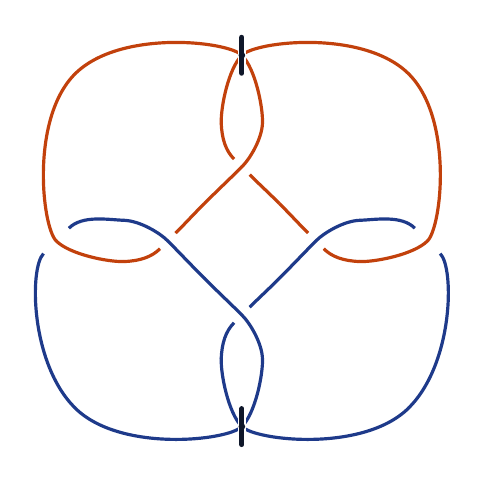
\begin{tikzpicture}[line join=round]
  \definecolor{skcomp0}{RGB}{30,58,138}
  \definecolor{skcomp1}{RGB}{194,65,12}
  \definecolor{skmark}{RGB}{15,23,42}
  \draw[skcomp0, line width=1.15pt, line cap=butt] (-2.1969,0.1610) .. controls (-2.0259,0.3320) and (-1.6992,0.2687) .. (-1.4977,0.2619);
  \draw[skcomp0, line width=1.15pt, line cap=butt] (-2.5189,-0.1610) .. controls (-2.7000,-0.3421) and (-2.6880,-1.5519) .. (-2.1200,-2.1200);
  \draw[skcomp1, line width=1.15pt, line cap=butt] (-1.0395,-0.0991) .. controls (-1.1448,-0.2043) and (-1.2962,-0.2551) .. (-1.4977,-0.2619);
  \draw[skcomp1, line width=1.15pt, line cap=butt] (-0.8414,0.0991) .. controls (-0.7316,0.2088) and (-0.6231,0.3283) .. (-0.4757,0.4757);
  \draw[skcomp1, line width=1.15pt, line cap=butt] (-0.0991,1.0395) .. controls (-0.2043,1.1448) and (-0.2551,1.2962) .. (-0.2619,1.4977);
  \draw[skcomp1, line width=1.15pt, line cap=butt] (0.0991,0.8414) .. controls (0.2088,0.7316) and (0.3283,0.6231) .. (0.4757,0.4757);
  \draw[skcomp1, line width=1.15pt, line cap=butt] (0.8414,0.0991) .. controls (0.7316,0.2088) and (0.6231,0.3283) .. (0.4757,0.4757);
  \draw[skcomp0, line width=1.15pt, line cap=butt] (2.5189,-0.1610) .. controls (2.7000,-0.3421) and (2.6880,-1.5519) .. (2.1200,-2.1200);
  \draw[skcomp0, line width=1.15pt, line cap=butt] (-0.0991,-1.0395) .. controls (-0.2043,-1.1448) and (-0.2551,-1.2962) .. (-0.2619,-1.4977);
  \draw[skcomp0, line width=1.15pt, line cap=butt] (0.0991,-0.8414) .. controls (0.2088,-0.7316) and (0.3283,-0.6231) .. (0.4757,-0.4757);
  \draw[skcomp1, line width=1.15pt, line cap=butt] (1.0395,-0.0991) .. controls (1.1448,-0.2043) and (1.2962,-0.2551) .. (1.4977,-0.2619);
  \draw[skcomp0, line width=1.15pt, line cap=butt] (2.1969,0.1610) .. controls (2.0259,0.3320) and (1.6992,0.2687) .. (1.4977,0.2619);
  \draw[skcomp0, line width=1.15pt, line cap=round] (-0.9405,-0.0000) .. controls (-1.0457,0.1052) and (-1.2962,0.2551) .. (-1.4977,0.2619);
  \draw[skcomp1, line width=1.15pt, line cap=round] (-2.3579,0.0000) .. controls (-2.5390,0.1811) and (-2.6880,1.5519) .. (-2.1200,2.1200);
  \draw[skcomp1, line width=1.15pt, line cap=round] (0.0000,2.3579) .. controls (-0.1811,2.5390) and (-1.5519,2.6880) .. (-2.1200,2.1200);
  \draw[skcomp0, line width=1.15pt, line cap=round] (0.0000,-2.3579) .. controls (-0.1811,-2.5390) and (-1.5519,-2.6880) .. (-2.1200,-2.1200);
  \draw[skcomp1, line width=1.15pt, line cap=round] (-2.3579,0.0000) .. controls (-2.1869,-0.1710) and (-1.6992,-0.2687) .. (-1.4977,-0.2619);
  \draw[skcomp0, line width=1.15pt, line cap=round] (-0.9405,-0.0000) .. controls (-0.8307,-0.1098) and (-0.6231,-0.3283) .. (-0.4757,-0.4757);
  \draw[skcomp0, line width=1.15pt, line cap=round] (0.0000,-0.9405) .. controls (-0.1098,-0.8307) and (-0.3283,-0.6231) .. (-0.4757,-0.4757);
  \draw[skcomp1, line width=1.15pt, line cap=round] (0.0000,0.9405) .. controls (-0.1098,0.8307) and (-0.3283,0.6231) .. (-0.4757,0.4757);
  \draw[skcomp1, line width=1.15pt, line cap=round] (0.0000,2.3579) .. controls (-0.1710,2.1869) and (-0.2687,1.6992) .. (-0.2619,1.4977);
  \draw[skcomp1, line width=1.15pt, line cap=round] (0.0000,2.3579) .. controls (0.1710,2.1869) and (0.2687,1.6992) .. (0.2619,1.4977);
  \draw[skcomp1, line width=1.15pt, line cap=round] (0.0000,0.9405) .. controls (0.1052,1.0457) and (0.2551,1.2962) .. (0.2619,1.4977);
  \draw[skcomp1, line width=1.15pt, line cap=round] (0.0000,2.3579) .. controls (0.1811,2.5390) and (1.5519,2.6880) .. (2.1200,2.1200);
  \draw[skcomp1, line width=1.15pt, line cap=round] (2.3579,-0.0000) .. controls (2.5390,0.1811) and (2.6880,1.5519) .. (2.1200,2.1200);
  \draw[skcomp0, line width=1.15pt, line cap=round] (0.0000,-2.3579) .. controls (0.1811,-2.5390) and (1.5519,-2.6880) .. (2.1200,-2.1200);
  \draw[skcomp0, line width=1.15pt, line cap=round] (0.0000,-2.3579) .. controls (0.1710,-2.1869) and (0.2687,-1.6992) .. (0.2619,-1.4977);
  \draw[skcomp0, line width=1.15pt, line cap=round] (0.0000,-0.9405) .. controls (0.1052,-1.0457) and (0.2551,-1.2962) .. (0.2619,-1.4977);
  \draw[skcomp0, line width=1.15pt, line cap=round] (0.0000,-2.3579) .. controls (-0.1710,-2.1869) and (-0.2687,-1.6992) .. (-0.2619,-1.4977);
  \draw[skcomp0, line width=1.15pt, line cap=round] (0.9405,-0.0000) .. controls (0.8307,-0.1098) and (0.6231,-0.3283) .. (0.4757,-0.4757);
  \draw[skcomp1, line width=1.15pt, line cap=round] (2.3579,-0.0000) .. controls (2.1869,-0.1710) and (1.6992,-0.2687) .. (1.4977,-0.2619);
  \draw[skcomp0, line width=1.15pt, line cap=round] (0.9405,-0.0000) .. controls (1.0457,0.1052) and (1.2962,0.2551) .. (1.4977,0.2619);
  \draw[white, line width=2.8pt, line cap=round] (0.0000,2.5856) -- (0.0000,2.1302);
  \draw[skmark, line width=1.85pt, line cap=round] (0.0000,2.5856) -- (0.0000,2.1302);
  \fill[skmark] (0.0000,2.3579) circle (1.2pt);
  \draw[white, line width=2.8pt, line cap=round] (0.0000,-2.1302) -- (0.0000,-2.5856);
  \draw[skmark, line width=1.85pt, line cap=round] (0.0000,-2.1302) -- (0.0000,-2.5856);
  \fill[skmark] (0.0000,-2.3579) circle (1.2pt);
\end{tikzpicture}
\end{document}
